\section{量子力学概要}

和量子化学无关的量子力学知识一概不讲。

更多内容见：
\begin{itemize}
  \item Levine 的 \textit{Quantum Chemistry} 7ed 前一半，有电子版；
  \item \textit{Introduction to Quantum Mechanics}（2ed, Griffiths），市面有影印版及习题解答。
\end{itemize}

更深入内容见：
\begin{itemize}
  \item \textit{Modern Quantum Mechanics}（Sakurai），市面有影印版。
\end{itemize}

经典力学（classical mechanics）适用于描述宏观粒子。它通过位置和速度来描述粒子的状态，其运动方程是牛顿方程。

微观粒子有明显的量子效应，需要改用量子力学（quantum mechanics, QM）研究。量子力学通过波函数（wavefunction）描述粒子的状态，粒子没有确定的位置，行为表现出波粒二象性，其运动方程是薛定谔方程（Schr\"odinger equation）。

\begin{center}
\begin{tikzpicture}[scale=0.95]
  \draw[->] (0,0) -- (5.8,0) node[right] {位置};
  \draw[->] (0,0) -- (0,2.9) node[above] {波函数值};
  \draw[line width=0.9pt, smooth] plot coordinates {
    (0.3,0.05) (0.8,0.08) (1.3,0.20) (1.8,0.75) (2.2,1.75)
    (2.6,2.35) (3.0,2.05) (3.4,1.15) (3.8,0.42) (4.3,0.10) (5.1,0.03)
  };
\end{tikzpicture}
\end{center}

薛定谔方程（单粒子、一维情形）

\begin{center}
\setlength{\fboxsep}{10pt}
\fbox{$\displaystyle i\hbar \frac{\partial \Psi}{\partial t}
=
-\frac{\hbar^2}{2m}\frac{\partial^2 \Psi}{\partial x^2}
+V\Psi$}
\end{center}

其中，$\Psi(x,t)$ 为波函数，$V(x,t)$ 为外势，$x$ 为坐标，$m$ 为粒子质量，$i$ 为虚数符号，$\hbar$ 为普朗克常数除以 $2\pi$。外势和初始状态确定了，粒子的波函数也就确定了。

Born 对波函数的概率解释：
\[
P(x,t)=|\Psi(x,t)|^2=\Psi(x,t)^*\Psi(x,t)
\]
表示 $t$ 时刻粒子在 $x$ 处出现的概率密度。
\[
\int_a^b |\Psi(x,t)|^2\,dx
\]
表示 $t$ 时刻在 $x=[a,b]$ 区间内粒子出现的总概率。

\begin{center}
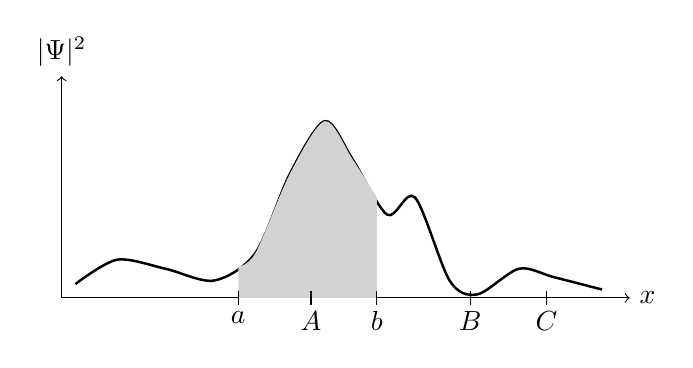
\begin{tikzpicture}[scale=0.88]
  \draw[->] (0,0) -- (8.2,0) node[right] {$x$};
  \draw[->] (0,0) -- (0,3.2) node[above] {$|\Psi|^2$};
  \draw[line width=0.9pt, smooth] plot coordinates {
    (0.2,0.20) (0.8,0.55) (1.5,0.42) (2.2,0.25) (2.8,0.65)
    (3.3,1.80) (3.8,2.55) (4.2,2.00) (4.7,1.20) (5.1,1.45)
    (5.6,0.25) (6.0,0.05) (6.6,0.42) (7.1,0.30) (7.8,0.12)
  };
  \fill[gray!35] (2.55,0) -- plot[smooth] coordinates {
    (2.55,0.45) (2.8,0.65) (3.3,1.80) (3.8,2.55) (4.2,2.00) (4.55,1.45)
  } -- (4.55,0) -- cycle;
  \draw (2.55,-0.10) -- (2.55,0.10) node[below=4pt] {$a$};
  \draw (4.55,-0.10) -- (4.55,0.10) node[below=4pt] {$b$};
  \draw (3.6,-0.10) -- (3.6,0.10) node[below=4pt] {$A$};
  \draw (5.9,-0.10) -- (5.9,0.10) node[below=4pt] {$B$};
  \draw (7.0,-0.10) -- (7.0,0.10) node[below=4pt] {$C$};
\end{tikzpicture}
\end{center}

有物理意义的波函数必须满足归一化条件：
\[
\int_{-\infty}^{+\infty} |\Psi(x,t)|^2\,dx = 1
\]

量子化学中用的波函数一般都是实数型，即
\[
\psi(x)=\psi(x)^*
\]

此时对于单粒子体系，在 $x$ 处出现的概率密度简写为
\[
P(x)=[\psi(x)]^2
\]

当 $V$ 与 $t$ 无关，则体系处于稳态，波函数可写为
\[
\Psi(x,t)=\psi(x)e^{-iEt/\hbar}
\]

对应的概率密度与时间无关，即
\[
|\Psi(x,t)|^2=\Psi^*\Psi=\psi^*e^{iEt/\hbar}\psi e^{-iEt/\hbar}=\psi^*\psi=|\psi(x)|^2
\]

此时薛定谔方程转化为不含时（time-independent）的形式，也称为定态薛定谔方程：

\begin{center}
\setlength{\fboxsep}{10pt}
\fbox{$\displaystyle E\psi=-\frac{\hbar^2}{2m}\frac{d^2\psi}{dx^2}+V\psi$}
\end{center}

其中 $E$ 为体系能量。后面课程涉及的一律为不含时的情况。

算符（operator）用于对它右侧的函数进行某种操作，一般用 $\hat{\ }$（hat）来表明。例如
\[
\hat A=\frac{d}{dx}, \qquad \hat A x^{3/4}=\frac{d\,x^{3/4}}{dx}=\frac{3}{4}x^{-1/4}
\]

算符本身也可以是个函数或常数，例如
\[
\hat A=x, \qquad \hat A x^{3/4}=x^{7/4}
\]

当算符中涉及微分时，和右侧的函数不能互换，即
\[
\hat A f(x)\neq f(x)\hat A
\]

亦不可从等号左右约掉函数，如
\[
\hat A f(x)=C f(x)
\]
不意味着
\[
\hat A=C
\]

对某个函数 $f$ 和常数 $C$，有如下关系时
\[
\hat A f=Cf
\]
$f$ 称为算符 $\hat A$ 的本征函数，$C$ 是其对应的本征值。

对本征函数乘上任意一个常数不会影响它对应的本征值。因此，为了物理意义清楚，一般会给该函数乘以一个因子使之满足归一化条件。

不同的算符对应不同的物理量，不同算符的本征函数集既可以相同也可以不同。

\begin{center}
\renewcommand{\arraystretch}{1.45}
\begin{tabular}{|>{\centering\arraybackslash}p{0.38\textwidth}|>{\centering\arraybackslash}p{0.20\textwidth}|>{\centering\arraybackslash}p{0.16\textwidth}|}
\hline
算符 & 本征函数 & 本征值 \\
\hline
位置算符 $\hat x$ & $\delta(x-x_0)$ & 位置 $x_0$ \\
\hline
动量算符 $\hat p=-i\hbar\dfrac{d}{dx}$ & $e^{ipx/\hbar}$ & 动量 $p$ \\
\hline
动能算符 $\hat T=\dfrac{\hat p\hat p}{2m}=-\dfrac{\hbar^2}{2m}\dfrac{d^2}{dx^2}$ & 同上 & 动能 $p^2/(2m)$ \\
\hline
角动量平方算符 $\hat l^2$ & 球谐函数 & 角动量平方 \\
\hline
哈密顿算符 $\hat H$ & 体系波函数 & 体系能量 \\
\hline
\end{tabular}
\end{center}

位置、动量、动能对应连续谱；角动量平方和体系能量对应离散谱。

如果一个波函数不是某算符的本征函数，那么对此算符对应的属性进行一次观测的话，波函数就会坍塌为此算符的某个本征函数，并且观测到的本征值就是这个本征函数对应的本征值。

例如对一个波函数的位置（对应坐标算符 $\hat x$）进行观测，如果观测到粒子出现在 $x=k$ 的位置，那么波函数就会坍塌为 $\delta(x-k)$。

\begin{center}
\begin{tikzpicture}[scale=0.9]
  \draw[->] (0,0) -- (4.5,0);
  \draw[line width=0.9pt, smooth] plot coordinates {
    (0.3,0.25) (0.9,0.35) (1.5,1.6) (2.0,0.55) (2.5,1.0) (3.0,0.7) (3.6,0.18) (4.1,0.05)
  };
  \draw[->, line width=0.8pt] (5.1,0.9) -- (6.4,0.9);
  \draw[->] (7.0,0) -- (11.0,0);
  \draw[line width=1.0pt] (9.0,0) -- (9.0,2.1);
  \node[below] at (9.0,0) {$k$};
\end{tikzpicture}
\end{center}

哈密顿算符（Hamiltonian operator）包含动能算符 $\hat T$ 和势能算符 $\hat V$ 两部分：
\[
\hat H=\hat T+\hat V
\]

动能算符形式是固定的，如单粒子、一维情形时为
\[
\hat T=-\frac{\hbar^2}{2m}\frac{d^2}{dx^2}
\]

势能算符一般是函数，根据粒子实际所处环境而定。例如，粒子受到中心在原点处的谐振势：
\[
\hat V=\frac{1}{2}kx^2=\frac{1}{2}m\nu^2x^2
\]

电子受到中心在 $x_0$ 处核电荷为 $Z$ 的吸引势：
\[
\hat V=-\frac{Z}{|x-x_0|}
\]

精确求解稳态薛定谔方程 $\hat H\psi=E\psi$ 得到的波函数是 $\hat H$ 的本征函数，本征值是体系能量。此方程往往不止一个解，满足
\[
\hat H \psi_n = E_n \psi_n
\]

能量最低的解称为基态，其余的都是激发态。

若 $E_i=E_j$，则 $i$、$j$ 两个态是能级简并的（degenerate）。

只要有了哈密顿算符的具体形式，原理上就可以求解出体系的波函数，同时得到体系能量，还能进一步求得体系一切其它性质。求解薛定谔方程是量子力学的最关键的问题。

一维谐振子（harmonic oscillator）是最简单的量子力学体系之一，其薛定谔方程为
\[
E\psi=\hat H\psi=\left(-\frac{\hbar^2}{2m}\frac{d^2}{dx^2}+\frac{1}{2}kx^2\right)\psi
\]

对于这样外势函数相对简单的情况可以解析地求解。其能量本征值为
\[
E_n=\left(n+\frac{1}{2}\right)h\nu
\]
其中频率
\[
\nu=\sqrt{k/m}
\]
\[
n=0,1,2,\ldots
\]
$n$ 称为量子数。

其本征函数可写为
\[
\psi_n(x)=\left(\frac{m\nu}{\pi\hbar}\right)^{1/4}\frac{1}{\sqrt{2^n n!}}\,H_n(\xi)e^{-\xi^2/2}
\]
其中
\[
\xi=\sqrt{\frac{m\nu}{\hbar}}\,x
\]

$\{\psi_n\}$ 是 $\hat H$ 的本征函数集合。$n=0$ 对应基态，$n\ge 1$ 对应激发态。

基态时谐振子体系能量不为 $0$，此能量称为零点能（zero point energy, ZPE）：
\[
E_0=\frac{1}{2}h\nu
\]

能解析求解的情况实在太少，大多数定态情况只能通过数值方法近似求解薛定谔方程。

\begin{center}
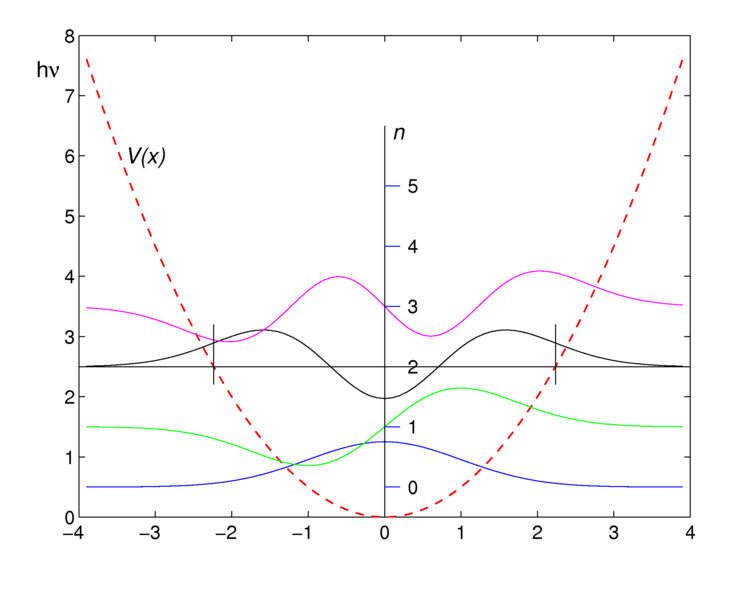
\includegraphics[width=0.47\textwidth]{assets/oscillator_wavefunctions.png}\hfill
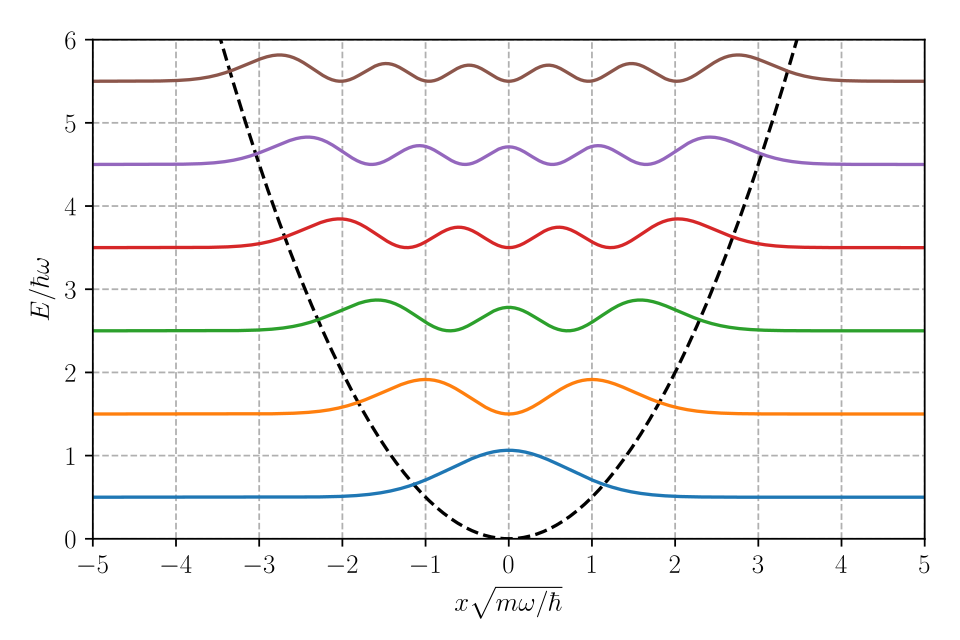
\includegraphics[width=0.47\textwidth,trim=40 30 40 35,clip]{assets/oscillator_probability_densities.png}
\end{center}

如果一个波函数是某个算符的本征函数，那么对此算符相应的属性进行观测，得到的就是其对应的本征值。

如果一个波函数不是某个算符的本征函数，那么每次对它的相应的物理量进行观测可能会得到不同的值。若进行大量观测，所观测到的平均值称为期望值，计算方式为
\[
\langle A\rangle=\int_{-\infty}^{+\infty}\psi(x)^*\,\hat A\,\psi(x)\,dx
\]

例如，实际中粒子的波函数都不是坐标算符的本征函数。若对粒子位置进行大量观测，得到的平均值即为
\[
\langle x\rangle
=
\int_{-\infty}^{+\infty}\psi(x)^*\,x\,\psi(x)\,dx
=
\int_{-\infty}^{+\infty}x\psi(x)^*\psi(x)\,dx
=
\int_{-\infty}^{+\infty}xP(x)\,dx
\]

相当于将坐标乘以相应位置粒子出现概率，然后全空间求和。

当然，若一个波函数本来就是某算符的本征函数，则期望值就是其本征值，如
\[
\langle H\rangle
=
\int_{-\infty}^{+\infty}\psi(x)^*\,\hat H\,\psi(x)\,dx
=
\int_{-\infty}^{+\infty}\psi(x)^*\,E\psi(x)\,dx
\]
\[
=
E\int_{-\infty}^{+\infty}\psi(x)^*\psi(x)\,dx
=
E
\]

有些算符是享有共同的本征函数集的，此时这两个算符间是对易的，即满足
\[
[\hat A,\hat B]=\hat A\hat B-\hat B\hat A=0
\]
即
\[
\hat A\hat B=\hat B\hat A
\]

对易的两个算符对应的两种物理量才是可以同时确定的。例如类氢原子波函数，既是角动量平方算符的本征函数，又是哈密顿算符的本征函数，所以既有确定的角动量平方值，又有确定的能量。

不对易的两个算符对应的两种物理量无法同时确定，如粒子的位置和动量无法同时确定（不确定原理，$\sigma_x\sigma_p\ge \hbar/2$）。

利用狄拉克符号（Dirac notation）不仅可以将量子力学中的积分表达大为简化，对于量子力学理论发展也有特殊意义。

右矢（ket）
\[
|\psi\rangle=\psi(x)
\]

左矢（bra）
\[
\langle \psi|=\int \psi(x)^*[\ldots]\,dx
\]

内积满足
\[
\langle \psi_i|\psi_j\rangle=\int_{-\infty}^{+\infty}\psi_i(x)^*\psi_j(x)\,dx
\]
\[
\langle \psi_i|\psi_j\rangle^*=\langle \psi_j|\psi_i\rangle
\]

算符矩阵元可写为
\[
\langle \psi_i|\hat A|\psi_j\rangle
=
\langle \psi_i|\hat A\psi_j\rangle
=
\int_{-\infty}^{+\infty}\psi_i(x)^*\,\hat A\,\psi_j(x)\,dx
\]

波函数对于某个算符的期望值写作
\[
\langle \psi|\hat A|\psi\rangle
\]

归一化条件
\[
\langle \psi|\psi\rangle=1
\]

正交条件
\[
\langle \psi_i|\psi_j\rangle=0
\]

实际可观测的物理量必定是实数，即
\[
y=y^*
\]

量子力学中，对应于可观测物理量的算符是厄米算符（Hermitian operator）。厄米算符满足
\[
\langle \Psi_i|\hat A\Psi_i\rangle=\langle \hat A\Psi_i|\Psi_i\rangle
\]
即
\[
\int \Psi_i(\mathbf r)^*\,\hat A\,\Psi_i(\mathbf r)\,d\mathbf r
=
\int [\hat A\Psi_i(\mathbf r)]^*\Psi_i(\mathbf r)\,d\mathbf r
\]

亦可由此推得更广义的关系
\[
\langle \Psi_i|\hat A|\Psi_j\rangle
\equiv
\langle \hat A\Psi_i|\Psi_j\rangle
=
\langle \Psi_j|\hat A\Psi_i\rangle^*
\equiv
\langle \Psi_j|\hat A|\Psi_i\rangle^*
\]

动量算符、动能算符、势能算符、哈密顿算符等都是厄米算符。

厄米算符的拥有不同本征值的本征函数彼此间是正交的，具有相同本征值的本征函数（简并态）可以正交也可以不正交，不正交的时候也可以通过对它们线性组合得到彼此正交的本征函数。

例如，量子化学 HF 方法计算产生的分子轨道是 Fock 算符（一种单电子哈密顿算符）的本征函数，本征值是分子轨道能量，故能量不同的分子轨道间必定是正交的。

多电子原子体系无法精确求解薛定谔方程。但是如果只有一个原子核和一个电子，即类氢原子体系，是可以精确求解的，解得的波函数称为原子轨道。

\[
\hat H=-\frac{\hbar^2}{2m_e}\nabla^2-\frac{Ze^2}{4\pi\varepsilon_0 r}
\]

其中 $e$ 为 elementary charge，即质子所带电量，$Z$ 为核电荷数。

求解时需要通过分离变量，将径向和角度部分分离独立求解。

对多电子原子体系，若将电子间相互作用以平均场方式近似考虑，还是可以求解得到原子轨道的，显然结果和类氢原子轨道有一定差异。

原子轨道波函数可写为
\[
\psi_{nlm}\equiv R_{nl}(r)Y_{lm}(\theta,\varphi)
\]
其中 $R_{nl}(r)$ 是径向部分，$Y_{lm}(\theta,\varphi)$ 是角度部分（球谐函数）。

主量子数
\[
n=1,2,3,\ldots
\]

角量子数
\[
l=0,1,2,\ldots,n-1
\]
共 $n$ 个。

磁量子数
\[
m=-l,-l+1,\ldots,0,\ldots,l-1,l
\]
共 $2l+1$ 个。

对于类氢原子，$n$ 决定轨道能量：
\[
E_n=-\frac{Z^2}{2n^2}\ \text{Hartree}
\]

对于多电子原子，$n$ 和 $l$ 共同决定轨道能量。无外磁场时，每个 $(n,l)$ 壳层的 $2l+1$ 个不同磁量子数的轨道能量简并；而有外磁场时，由于 $2l+1$ 个轨道与磁场相互作用能不同，能量将发生分裂。

求解原子的薛定谔方程得到的原子轨道是角动量 $z$ 分量算符 $\hat L_z$ 的本征函数，有的是实函数，有的是复函数，后者不好进行描述和利用。由于每个壳层 $2l+1$ 个轨道能量简并，可以将它们适当线性组合产生出实数型原子轨道波函数，且能量不变。

\[
l=0
\]
称 $s$ 轨道，磁量子数仅为 $0$，只有 $1$ 个轨道。

\[
l=1
\]
称 $p$ 轨道，有 $3$ 个磁量子数，可组合出 $p_x$、$p_y$、$p_z$。

\[
l=2
\]
称 $d$ 轨道，有 $5$ 个磁量子数，可组合出 $d_{xy}$、$d_{yz}$、$d_{xz}$、$d_{x^2-y^2}$、$d_{z^2}$。

\[
l=3
\]
称 $f$ 轨道，有 $7$ 个磁量子数，可组合出 $7$ 个实数型轨道。

在线观看原子轨道图形的程序：$n$ 最高到 $12$，$l$ 最高到 $11$。
\[
\texttt{https://al2me6.github.io/evanescence/}
\]

原子轨道在径向上有 $n-l-1$ 个节点，相应地在径向分布函数上有 $n-l-1$ 个极小点。

\[
1s,\ \text{即 } n=1,\ l=0
\]
\[
2s,\ \text{即 } n=2,\ l=0
\]
\[
2p,\ \text{即 } n=2,\ l=1
\]

实数型原子轨道的角度部分常见为 $s$ 轨道、$p$ 轨道、$d$ 轨道和 $f$ 轨道。

三维、多粒子体系的哈密顿算符可写为
\[
\hat H
=
\sum_i^N\left[-\frac{\hbar^2}{2m_i}\nabla_i^2+V_i(\mathbf r_i)\right]
+
\sum_{i>j}^N V_{ij}(\mathbf r_i,\mathbf r_j)
\]

其中拉普拉斯算符
\[
\nabla_i^2=\frac{d^2}{dx_i^2}+\frac{d^2}{dy_i^2}+\frac{d^2}{dz_i^2}
\]

对应的薛定谔方程为
\[
\hat H\Psi(\mathbf r_1,\mathbf r_2,\ldots,\mathbf r_N)
=
E\Psi(\mathbf r_1,\mathbf r_2,\ldots,\mathbf r_N)
\]

除个别例外，多粒子体系的薛定谔方程从原理上无法解析地求解，只能通过数值方法近似求解。

同时在 $\mathbf r_1'$、$\mathbf r_2'$、$\ldots$、$\mathbf r_N'$ 处都发现一个粒子的概率为
\[
\rho(\mathbf r_1',\mathbf r_2',\cdots,\mathbf r_N')
=
\left|\Psi(\mathbf r_1',\mathbf r_2',\cdots,\mathbf r_N')\right|^2
\]

其归一化条件为
\[
\idotsint \rho(\mathbf r_1,\mathbf r_2,\ldots,\mathbf r_N)\,d\mathbf r_1\,d\mathbf r_2\cdots d\mathbf r_N=1
\]

在 $\mathbf r_1'$、$\mathbf r_2'$ 处都发现一个粒子的概率，而不管其它位置什么情况，为
\[
\rho(\mathbf r_1',\mathbf r_2')
=
N(N-1)\int\cdots\int
\left|\Psi(\mathbf r_1',\mathbf r_2',\ldots,\mathbf r_N)\right|^2
\,d\mathbf r_3\cdots d\mathbf r_N
\]

在 $\mathbf r_1'$ 处发现一个粒子的概率，即单粒子密度，为
\[
\rho(\mathbf r_1')
=
N\int\cdots\int
\left|\Psi(\mathbf r_1',\mathbf r_2,\ldots,\mathbf r_N)\right|^2
\,d\mathbf r_2\,d\mathbf r_3\cdots d\mathbf r_N
\]

对于一个多粒子体系，如果粒子之间没有相互作用（独立粒子），那么整体的波函数可以写为各个波函数的乘积：
\[
\Psi(\mathbf r_1,\mathbf r_2,\cdots,\mathbf r_N)=\psi(\mathbf r_1)\psi(\mathbf r_2)\cdots\psi(\mathbf r_N)
\]

体系总哈密顿是这些独立粒子哈密顿之和：
\[
\hat h_i\psi_i=\varepsilon_i\psi_i
\]
\[
\hat H=\sum_i \hat h_i
\]

体系总能量也是独立粒子能量之和：
\[
E=\sum_i \varepsilon_i
\]

分子体系的电子哈密顿算符中，一般不考虑原子核的量子效应，而把原子核视为有确定位置 $\mathbf R$ 的点电荷。只把电子以量子力学方式考虑。电子的哈密顿为
\[
\hat H_{\mathrm{ele}}
=
\sum_i\left[
-\frac{\hbar^2}{2m_e}\nabla_i^2
-\sum_A\frac{Z_Ae^2}{4\pi\varepsilon_0 r_{iA}}
\right]
+
\sum_{i>j}\frac{e^2}{4\pi\varepsilon_0 r_{ij}}
\]

其中 $r_{iA}$ 是电子 $i$ 与核 $A$ 的距离，$r_{ij}$ 是电子 $i$ 与电子 $j$ 的距离。

原子单位（a.u.）将 $m_e$、$e$、$\hbar$、库仑常数 $1/(4\pi\varepsilon_0)$ 定义为 $1$，使得公式简化许多：
\[
\hat H_{\mathrm{ele}}
=
\sum_i\left[
-\frac{1}{2}\nabla_i^2
-\sum_A\frac{Z_A}{r_{iA}}
\right]
+
\sum_{i>j}\frac{1}{r_{ij}}
\]

体系总哈密顿可以写为
\[
\hat H_{\mathrm{tot}}=\hat H_{\mathrm{ele}}+\hat V_{NN}
\]

在特定的几何坐标下，体系能量等于电子能量与核互斥势能的加和：
\[
E_{\mathrm{tot}}
=(T_{\mathrm{ele}}+V_{\mathrm{ele}})+V_{NN}
=
E_{\mathrm{ele}}+V_{NN}
\]
\[
=
\langle \psi_{\mathrm{ele}}|\hat H_{\mathrm{ele}}|\psi_{\mathrm{ele}}\rangle
+
\sum_{B>A}\frac{Z_AZ_B}{R_{AB}}
\]

量子化学的通用语言中，“电子能量”就是指上式体系总能量 $E_{\mathrm{tot}}$，而非仅仅 $E_{\mathrm{ele}}$ 这一项。

线性组合（linear combination）

对于一个复杂的函数，可以将它写为一套基函数的线性组合的形式，从而便于描述或求解。选用的基函数应当与被展开的函数有相同的边界条件。

\[
|f\rangle \approx \sum_i c_i |g_i\rangle
\]

如果基函数是彼此正交的，则组合系数 $c_i$ 可以通过令向量做投影来得到：
\[
c_i=\langle g_i|f\rangle
\]

完备集（complete set）

如果有一套基函数能够令某个函数被完美地线性展开，则这套基函数对它来说构成完备集。

厄米算符的所有本征函数可以作为完备集来展开与之具有相同边界条件的任何函数。

谐振子体系哈密顿算符的本征函数可以线性组合起来，用来更精确地描述具有相同边界条件的其它函数。

线性变分法（linear variation method）

实际体系的势函数往往比较复杂，导致薛定谔方程不可能直接求解。一个极有用的近似求解方法是线性变分法。即人为地设定一套数学形式比较简单的基函数，记为 $\{\chi\}$，共 $N$ 个，令体系函数对其线性展开来近似地描述：
\[
\Psi \approx \sum_{i=1}^N C_i\chi_i
\]

体系能量
\[
E=\langle \Psi|\hat H|\Psi\rangle
\]

令 $E$ 对这些组合系数的偏导为 $0$：
\[
\frac{\partial E}{\partial C_i}=0,\qquad i=1,2,3,\ldots,N
\]

同时通过拉格朗日乘子法约束它满足归一化条件，就可以找到参数空间 $\{C\}$ 的极值点，即薛定谔方程在当前基函数集下的最优的近似解。所得的各个解满足如下条件：
\[
E_{\mathrm{real}}\le E_1\le E_2\le \cdots \le E_N
\]

$E_{\mathrm{real}}$ 为体系真正基态能量。变分法得到的能量不会比它更低，称为变分原理（variation principle）。

由于限于计算量，实际计算时设定的基函数的数目肯定是有限的，因此通过线性变分法得到的只是近似的解，$E_1$ 必高于真实基态能量。基函数给得越多、越合适，解就越精确，$E_1$ 就越接近真实基态能量。当基函数无穷多时（完备集），$E_1=E_{\mathrm{real}}$。

可以证明，如果给定的 $N$ 个基函数是正交归一的，那么对体系能量进行线性变分，等价于求解如下矩阵本征方程：
\[
\mathbf H\mathbf C=\mathbf C\mathbf E
\]

其中
\[
H_{ij}=\langle \chi_i|\hat H|\chi_j\rangle
\]

求解此方程实际上就是将哈密顿矩阵 $\mathbf H$ 对角化，得到系数矩阵 $\mathbf C$ 和能量矩阵 $\mathbf E$。

\[
C_{mn}
\]
矩阵元对应第 $n$ 个解当中第 $m$ 个基函数的组合系数。

\[
\mathbf E
\]
是对角矩阵，$E_i$ 就是体系的第 $i$ 个解的能量。

求解薛定谔方程从原理上来讲并非难事，线性变分法提供了直接可行的求解对策。量子化学之所以理论、算法复杂且种类繁多，一方面在于会牵扯到电子积分计算等复杂数学问题，一方面牵扯到复杂编程问题，还一方面在于人们不断寻求能以更低的计算量达到更好精度的方法。

维里定理（Virial theorem）

对多原子体系，当原子核受力为 $0$ 时，对于精确波函数，或完备基组下完全以变分方式得到的波函数，如 HF、MCSCF 波函数，势能和动能满足如下关系：
\[
2T_{\mathrm{ele}}=-V_{\mathrm{tot}}=-(V_{\mathrm{ele}}+V_{NN})
\]

维里比值理想值：
\[
-\frac{V_{\mathrm{tot}}}{T_{\mathrm{ele}}}=2
\]

体系总能量：
\[
E_{\mathrm{tot}}=T_{\mathrm{ele}}+V_{\mathrm{tot}}=-T_{\mathrm{ele}}=\frac{V_{\mathrm{tot}}}{2}
\]

Hellmann-Feynman 定理

对于实际精确波函数，或完全变分法得到的波函数且用的基函数不依赖于核坐标，$i$ 原子核（坐标为 $R_i$）的受力可简单写为
\[
F_i=-\frac{\partial E}{\partial R_i}
=
\frac{\partial \langle \Psi|\hat H_{\mathrm{tot}}|\Psi\rangle}{\partial R_i}
=
\left\langle \Psi\left|\frac{\partial \hat H_{\mathrm{tot}}}{\partial R_i}\right|\Psi\right\rangle
\]

满足 Hellmann-Feynman 定理的理论方法在计算原子受力时会比较容易，否则还会额外牵扯到波函数对核坐标的导数项。

电子自旋（electron spin）

不考虑旋轨耦合的情况下，电子波函数可以写为空间部分与自旋部分的乘积：
\[
\psi(\mathbf r;\omega)=\varphi(\mathbf r)\sigma(\omega)
\]

其中 $\varphi$ 为空间函数，$\mathbf r$ 为空间坐标；$\sigma$ 为自旋函数，$\omega$ 为自旋坐标。

电子有 $\alpha$ 和 $\beta$ 两种自旋，对应两种自旋函数，彼此正交：
\[
\sigma(\omega)\in
\left\{
\alpha(\omega),\,
\beta(\omega)
\right\}
\]
\[
\langle \sigma_i|\sigma_j\rangle \equiv \int \sigma_i(\omega)\sigma_j(\omega)\,d\omega
\]
\[
\langle \alpha|\alpha\rangle=1,\qquad
\langle \beta|\beta\rangle=1,\qquad
\langle \alpha|\beta\rangle=0
\]

$\alpha$ 和 $\beta$ 电子的自旋量子数 $s$ 都为 $1/2$，但自旋磁量子数 $m_s$ 分别为 $1/2$ 和 $-1/2$：
\[
\sigma\equiv |s,m_s\rangle,\qquad
\alpha\equiv\left|\frac{1}{2},\frac{1}{2}\right\rangle,\qquad
\beta\equiv\left|\frac{1}{2},-\frac{1}{2}\right\rangle
\]

自旋函数是自旋角动量平方算符和自旋角动量在某一方向分量（一般取 $z$）算符的本征函数：
\[
\hat S^2|s,m_s\rangle=s(s+1)|s,m_s\rangle
\]
\[
\hat S_z|s,m_s\rangle=m_s|s,m_s\rangle
\]

对于多电子体系，自旋部分函数是总自旋角动量平方算符和某一方向分量算符的本征函数：
\[
\hat S^2|S,M_S\rangle=S(S+1)|S,M_S\rangle
\]
\[
\hat S_z|S,M_S\rangle=M_S|S,M_S\rangle
\]

体系如果有 $N$ 个 $\alpha$ 电子、$M$ 个 $\beta$ 电子，那么体系总自旋量子数就为
\[
S=\frac{N-M}{2}
\]
并且有 $2S+1$ 个分量，被称为自旋多重度。这些自旋态分别对应
\[
M_S=-S,-S+1,\ldots,S-1,S
\]

没有外加磁场时，$2S+1$ 个自旋态能量是简并的；而当有外加磁场时，由于电子自旋磁矩和磁场的作用不同，$2S+1$ 个自旋态的能量会发生分裂。

全同粒子体系与反对称原理

量子体系中同种粒子组成全同粒子体系。粒子之间彼此不可分辨，比如不能说第 $i$ 个、第 $j$ 个电子。

自然界粒子分为波色子（Boson）和费米子（Fermion）。费米子包括电子、质子、中子、夸克等；波色子包括光子、胶子、介子等。

费米子构成的全同粒子体系的波函数满足反对称原理，即交换两个费米子的坐标会导致波函数符号变号：
\[
\Psi(\mathbf r_1,\cdots,\mathbf r_i,\cdots,\mathbf r_j,\cdots,\mathbf r_N)
=
-\Psi(\mathbf r_1,\cdots,\mathbf r_j,\cdots,\mathbf r_i,\cdots,\mathbf r_N)
\]

对于波色子构成的波函数，这样交换则不会变号。

这也说明两个自旋相同的电子出现在同一个位置时波函数为 $0$，即概率为 $0$，因为只有 $0$ 才等于它的负值。

推论（Pauli 不相容原理）：两个或多个费米子不能同时处在同一个量子态。如果同时处于同一个量子态，那么它们至少也得有一个属性不同。一个分子轨道不能占据两个自旋相同的电子正是这个道理。
